\documentclass[11pt,a4paper]{article}

% ── Geometry & Layout ──
\usepackage[margin=2.5cm]{geometry}
\usepackage{parskip}

% ── Typography ──
\usepackage[T1]{fontenc}
\usepackage{lmodern}
\usepackage{microtype}

% ── Code Listings ──
\usepackage{listings}
\usepackage{xcolor}

\definecolor{codebg}{HTML}{F5F5F0}
\definecolor{codecomment}{HTML}{6A737D}
\definecolor{codekeyword}{HTML}{D73A49}
\definecolor{codestring}{HTML}{032F62}
\definecolor{codenumber}{HTML}{005CC5}
\definecolor{tipbg}{HTML}{E8F5E9}
\definecolor{tipframe}{HTML}{4CAF50}
\definecolor{warnbg}{HTML}{FFF3E0}
\definecolor{warnframe}{HTML}{FF9800}

\lstdefinestyle{cppstyle}{
  language=C++,
  backgroundcolor=\color{codebg},
  basicstyle=\ttfamily\small,
  keywordstyle=\color{codekeyword}\bfseries,
  commentstyle=\color{codecomment}\itshape,
  stringstyle=\color{codestring},
  numberstyle=\tiny\color{codenumber},
  numbers=left,
  numbersep=6pt,
  frame=single,
  rulecolor=\color{black!20},
  breaklines=true,
  tabsize=2,
  showstringspaces=false,
  morekeywords={glm,vec3,vec4,mat4,uint32_t,uint8_t,int16_t,size_t,float,
                SDL_GPUDevice,SDL_GPUBuffer,SDL_GPUTexture,SDL_GPUSampler,
                SDL_GPUCommandBuffer,SDL_GPURenderPass,SDL_Window,
                std,vector,string,function,atomic,span,unordered_map,
                flecs,world}
}

\lstdefinestyle{glslstyle}{
  language=C,
  backgroundcolor=\color{codebg},
  basicstyle=\ttfamily\small,
  keywordstyle=\color{codekeyword}\bfseries,
  commentstyle=\color{codecomment}\itshape,
  stringstyle=\color{codestring},
  frame=single,
  rulecolor=\color{black!20},
  breaklines=true,
  tabsize=2,
  showstringspaces=false,
  morekeywords={layout,set,binding,uniform,buffer,readonly,writeonly,
                local_size_x,local_size_y,local_size_z,
                vec2,vec3,vec4,mat4,uint,uvec3,ivec2,
                in,out,flat,location,push_constant}
}

\lstset{style=cppstyle}

% ── Diagrams ──
\usepackage{tikz}
\usetikzlibrary{positioning,arrows.meta,shapes.geometric,fit,calc,backgrounds}

% ── Callout Boxes ──
\usepackage[most]{tcolorbox}
\newtcolorbox{howtip}{
  colback=tipbg, colframe=tipframe,
  fonttitle=\bfseries, title={How to Recreate},
  arc=2mm, boxrule=0.8pt, left=4pt, right=4pt, top=2pt, bottom=2pt
}
\newtcolorbox{warnbox}{
  colback=warnbg, colframe=warnframe,
  fonttitle=\bfseries, title={Important},
  arc=2mm, boxrule=0.8pt, left=4pt, right=4pt, top=2pt, bottom=2pt
}

% ── Tables ──
\usepackage{booktabs}
\usepackage{array}
\usepackage{longtable}

% ── Cross-references ──
\usepackage[colorlinks=true,linkcolor=blue!60!black,urlcolor=blue!60!black,citecolor=blue!60!black]{hyperref}
\usepackage{cleveref}

% ── Math ──
\usepackage{amsmath}

% ══════════════════════════════════════════════════════════════════════
\title{\textbf{Delve Architectural Blueprint}\\[0.4em]
       \large A Comprehensive Guide to Recreating Every System}
\author{Delve Project}
\date{March 2026}

\begin{document}
\maketitle
\tableofcontents
\newpage

% ══════════════════════════════════════════════════════════════════════
\section{Project Overview \& Build System}
\label{sec:overview}

Delve is a procedural hex-grid terrain generator written in C++20. It renders isometric 3D landscapes using layered Perlin/Worley noise with real-time parameter editing via ImGui. The GPU backend uses SDL3-GPU, which abstracts over Vulkan, Metal, and DirectX~12.

\subsection{Prerequisites}

\begin{itemize}
  \item \textbf{SDL3} --- system package (windowing, GPU abstraction)
  \item \textbf{glslc} --- SPIR-V shader compiler (from Vulkan SDK or shaderc)
  \item \textbf{CMake} $\geq$ 3.20
  \item A C++20-capable compiler
\end{itemize}

\subsection{Build Commands \& Targets}

\begin{lstlisting}[style=cppstyle,language=bash,numbers=none]
cmake -B build -DCMAKE_BUILD_TYPE=Release   # configure
cmake --build build -j$(nproc)              # build all
./build/topogen                             # run application
cmake --build build --target delve_tests    # build tests
./build/delve_tests                         # run tests (JSON to stdout)
\end{lstlisting}

\begin{table}[h]
\centering
\caption{CMake build targets}
\label{tab:targets}
\begin{tabular}{@{}llp{7cm}@{}}
\toprule
\textbf{Target} & \textbf{Type} & \textbf{Description} \\
\midrule
\texttt{imgui}         & Static lib  & ImGui core + SDL3/SDL-GPU backends \\
\texttt{topo\_engine}  & Static lib  & Reusable engine framework (18 source files) \\
\texttt{topogen}       & Executable  & Main application (21 game sources) \\
\texttt{delve\_tests}  & Executable  & Headless test runner (\texttt{EXCLUDE\_FROM\_ALL}) \\
\texttt{delve\_metrics}& Executable  & Headless metrics binary (\texttt{EXCLUDE\_FROM\_ALL}) \\
\texttt{shaders}       & Custom      & GLSL $\to$ SPIR-V compilation \\
\bottomrule
\end{tabular}
\end{table}

\subsection{Dependency Management}

\begin{table}[h]
\centering
\caption{External dependencies}
\label{tab:deps}
\begin{tabular}{@{}lllp{5.5cm}@{}}
\toprule
\textbf{Library} & \textbf{Version} & \textbf{Method} & \textbf{CMake Target} \\
\midrule
Flecs          & v4.0.5  & FetchContent & \texttt{flecs::flecs\_static} \\
nlohmann/json  & v3.11.3 & FetchContent & \texttt{nlohmann\_json::nlohmann\_json} \\
GLM            & 1.0.1   & FetchContent & \texttt{glm::glm} \\
ImGui          & latest  & Git submodule & \texttt{imgui} (static lib) \\
cgltf          & latest  & Vendored header & \texttt{third\_party/cgltf/} \\
stb\_image     & latest  & Vendored header & \texttt{third\_party/stb/} \\
FastNoiseLite  & latest  & Vendored header & \texttt{src/game/terrain/} \\
\bottomrule
\end{tabular}
\end{table}

\subsection{Shader Compilation Pipeline}

Shaders are written in GLSL~4.5 in \texttt{src/shaders/} and compiled to SPIR-V via \texttt{glslc}. Three shared include files (\texttt{coord.glsl}, \texttt{lighting\_common.glsl}, \texttt{pbr\_common.glsl}) trigger a full rebuild of all dependents when modified.

\begin{lstlisting}[language=bash,numbers=none]
# Graphics shader compilation (per stage)
glslc -fshader-stage=vertex -I src/shaders/ -o build/shaders/X.spv src/shaders/X.glsl
# Compute shader compilation
glslc -fshader-stage=compute -I src/shaders/ -o build/shaders/X.spv src/shaders/X.glsl
\end{lstlisting}

Compile definitions propagated to C++: \texttt{SHADER\_DIR} (SPIR-V output path), \texttt{ASSET\_DIR} (project root \texttt{assets/}), \texttt{GLM\_FORCE\_DEPTH\_ZERO\_TO\_ONE}.

% ══════════════════════════════════════════════════════════════════════
\section{Engine Layer Architecture}
\label{sec:engine}

The engine lives in \texttt{src/engine/} and provides a reusable framework independent of game logic.

% ── Engine Architecture Diagram ──
\begin{figure}[h]
\centering
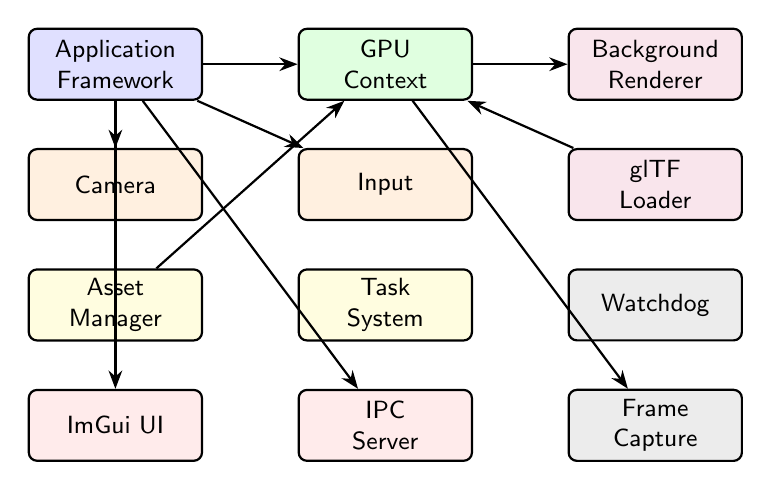
\begin{tikzpicture}[
  block/.style={rectangle, draw, rounded corners=3pt, minimum width=2.2cm,
                minimum height=0.9cm, align=center, font=\small\sffamily},
  >=Stealth, thick
]
  \node[block,fill=blue!12] (app)  {Application\\Framework};
  \node[block,fill=green!12, right=1.2cm of app]  (gpu)  {GPU\\Context};
  \node[block,fill=orange!12, below=0.6cm of app] (cam)  {Camera};
  \node[block,fill=orange!12, right=1.2cm of cam] (inp)  {Input};
  \node[block,fill=yellow!12, below=0.6cm of cam] (asset){Asset\\Manager};
  \node[block,fill=yellow!12, right=1.2cm of asset](task) {Task\\System};
  \node[block,fill=red!8,     below=0.6cm of asset](ui)  {ImGui UI};
  \node[block,fill=red!8,     right=1.2cm of ui]   (ipc) {IPC\\Server};
  \node[block,fill=purple!10, right=1.2cm of gpu]  (bg)  {Background\\Renderer};
  \node[block,fill=purple!10, right=1.2cm of inp]  (gltf){glTF\\Loader};
  \node[block,fill=gray!15,   right=1.2cm of task] (wd)  {Watchdog};
  \node[block,fill=gray!15,   right=1.2cm of ipc]  (fc)  {Frame\\Capture};

  \draw[->] (app) -- (gpu);
  \draw[->] (app) -- (cam);
  \draw[->] (app) -- (inp);
  \draw[->] (app) -- (ui);
  \draw[->] (app) -- (ipc);
  \draw[->] (gpu) -- (bg);
  \draw[->] (gpu) -- (fc);
  \draw[->] (asset) -- (gpu);
  \draw[->] (gltf) -- (gpu);
\end{tikzpicture}
\caption{Engine module dependency graph}
\label{fig:engine-arch}
\end{figure}

\subsection{Application Framework}
\label{sec:app}

\texttt{app.h/cpp} defines the abstract \texttt{Application} base class with a fixed-timestep main loop.

\textbf{Constants:}
\begin{itemize}
  \item \texttt{FIXED\_DT = 1/60\,s} (60\,FPS fixed timestep)
  \item \texttt{MAX\_FRAME\_TIME = 0.25\,s} (clamp to prevent spiral of death)
\end{itemize}

\textbf{Lifecycle hooks} (virtual methods overridden by the game):
\begin{itemize}
  \item \texttt{on\_init(GpuContext\&, flecs::world\&)}
  \item \texttt{on\_event(SDL\_Event\&, flecs::world\&)}
  \item \texttt{on\_render\_tool(GpuContext\&, FrameContext\&, flecs::world\&)} --- tool window (ImGui)
  \item \texttt{on\_render\_game(GpuContext\&, FrameContext\&, flecs::world\&)} --- game window (terrain)
  \item \texttt{on\_cleanup(flecs::world\&)}
\end{itemize}

\textbf{Main loop pseudocode:}
\begin{lstlisting}[numbers=none]
while (!quit) {
  poll_agent_server();          // IPC commands
  dt = clamp(elapsed, 0, MAX_FRAME_TIME);
  accumulator += dt;
  while (accumulator >= FIXED_DT) {
    ecs_world.progress(FIXED_DT);
    accumulator -= FIXED_DT;
  }
  poll_sdl_events();            // input, window events
  asset_manager.check_for_updates();  // shader hot-reload
  acquire_tool_frame();  on_render_tool();  end_frame();
  acquire_game_frame();  on_render_game();  end_frame();
}
\end{lstlisting}

\begin{howtip}
The dual-window setup renders ImGui controls in one window and the 3D viewport in another. Each window gets its own swapchain acquisition and render pass. The tool window is always rendered; the game window is conditional on \texttt{wants\_game\_window\_open()}.
\end{howtip}

\subsection{GPU Abstraction}
\label{sec:gpu}

\texttt{gpu/gpu.h/cpp} wraps SDL3-GPU with higher-level upload and frame management.

\textbf{Key structures:}
\begin{lstlisting}
struct UploadManager {
  SDL_GPUTransferBuffer *buffer;   // persistent 8 MB staging buffer
  uint8_t *mapped;                 // persistently mapped CPU pointer
  uint32_t capacity;               // 8 * 1024 * 1024
  uint32_t cursor;                 // current write offset
  // alloc(): 256-byte aligned bump allocation
  // reset(): cursor = 0 at frame start
};

struct GpuContext {
  SDL_Window *window, *game_window;
  SDL_GPUDevice *device;
  UploadManager upload_manager;
};

struct FrameContext {
  SDL_GPUCommandBuffer *cmd;
  SDL_GPUTexture *swapchain;
  SDL_GPURenderPass *render_pass;
  uint32_t swapchain_w, swapchain_h;
};
\end{lstlisting}

\textbf{Buffer utilities:}
\begin{itemize}
  \item \texttt{gpu\_create\_buffer()} --- allocates GPU buffer with usage flags
  \item \texttt{gpu\_upload\_buffer()} --- creates buffer and uploads data in one call
  \item \texttt{upload\_rgba\_texture()} --- creates sRGB or linear texture with REPEAT sampler
\end{itemize}

\begin{howtip}
The UploadManager uses a single 8\,MB transfer buffer with bump allocation (256-byte aligned). This avoids per-frame buffer creation overhead. Reset the cursor to zero at the start of each game frame, not the tool frame.
\end{howtip}

\subsection{Camera System}
\label{sec:camera}

The isometric camera in \texttt{camera/camera.h/cpp} uses a custom projection combining 2:1 tile aspect with height scaling.

\textbf{Isometric constants:}
\begin{align}
  \text{TW} &= 2.0 \quad \text{(tile width scale, X axis)} \\
  \text{TH} &= 1.0 \quad \text{(tile height scale, Y axis)} \\
  \text{HS} &= 12.5 \quad \text{(height scale = ISO\_HEIGHT\_SCALE / HEX\_SIZE)}
\end{align}

\textbf{Coordinate transform} (world $\to$ isometric screen):
\begin{align}
  \text{iso}_x &= (w_x - w_y) \cdot \text{TW} \\
  \text{iso}_y &= (w_x + w_y) \cdot \text{TH} - w_z \cdot \text{HS} \\
  \text{iso}_z &= (w_x + w_y) \cdot \text{TH} + w_z \quad \text{(depth)}
\end{align}

\textbf{View matrix} (column-major):
\begin{lstlisting}
view = mat4(
  vec4( TW,  TH,  TH, 0),  // world X -> iso
  vec4(-TW,  TH,  TH, 0),  // world Y -> iso
  vec4(  0, -HS, 1.0, 0),  // world Z -> iso
  vec4(  0,   0,   0, 1)
);
\end{lstlisting}

\textbf{Follow smoothing} uses exponential decay: $t = 1 - e^{-\text{speed} \cdot dt}$, with default \texttt{follow\_speed = 5.0}. Orthographic projection uses \texttt{glm::ortho} with Y-flip (top $>$ bottom). Camera shake applies random offsets scaled by a linear fade-out.

\subsection{Input System}

\texttt{input/input.h} maps SDL scancodes to an \texttt{Action} enum (13 actions: MoveUp/Down/Left/Right, Interact, Cancel, Pause, ZoomIn/Out, CameraUp/Down/Left/Right). Tracks three states per action: \texttt{pressed} (single frame), \texttt{held}, \texttt{released} (single frame). Call \texttt{begin\_frame()} to clear transient flags.

\subsection{Asset Manager}
\label{sec:asset}

\texttt{core/asset\_manager.h/cpp} provides shader caching and hot-reload:
\begin{itemize}
  \item \texttt{load\_shader(key, path, stage, ...)} --- reads SPIR-V binary, caches by key
  \item \texttt{register\_pipeline(key, vert\_key, frag\_key)} --- tracks vert/frag dependency
  \item \texttt{check\_for\_updates()} --- polls file \texttt{stat()} for mtime changes each frame
  \item On change: sets \texttt{dirty=true} on shader, \texttt{needs\_rebuild=true} on dependent pipelines
\end{itemize}

\subsection{Task System}

\texttt{core/task\_system.h/cpp} implements a thread pool using \texttt{std::mutex + std::condition\_variable}. Workers wait on the CV, pick tasks from a deque, and decrement an \texttt{atomic<int> active\_count}. \texttt{is\_idle()} returns true when the queue is empty and active count is zero.

\subsection{Watchdog}

\texttt{core/watchdog.h/cpp} spawns a background thread that reads \texttt{/proc/self/status} for \texttt{VmRSS} every 500\,ms. Default limit: 75\% of total RAM (fallback 2\,GB). On breach, sets \texttt{g\_emergency\_shutdown = true} and calls \texttt{std::quick\_exit(1)} after a 500\,ms grace period.

\subsection{glTF Loader}
\label{sec:gltf}

\texttt{core/gltf\_loader.h/cpp} loads static meshes via cgltf and textures via stb\_image.

\begin{table}[h]
\centering
\caption{GltfVertex layout (48 bytes)}
\begin{tabular}{@{}llrl@{}}
\toprule
\textbf{Field} & \textbf{Type} & \textbf{Bytes} & \textbf{Offset} \\
\midrule
position & vec3  & 12 & 0  \\
normal   & vec3  & 12 & 12 \\
texcoord & vec2  &  8 & 24 \\
tangent  & vec4  & 16 & 32 \\
\bottomrule
\end{tabular}
\end{table}

\textbf{cgltf functions used:} \texttt{cgltf\_parse\_file()}, \texttt{cgltf\_load\_buffers()}, \texttt{cgltf\_validate()}, \texttt{cgltf\_accessor\_read\_float()}, \texttt{cgltf\_accessor\_read\_uint()}.

\subsection{ImGui Integration}

Custom SDL3-GPU backends (submodule in \texttt{imgui/}). Six-function API: \texttt{ui\_init}, \texttt{ui\_shutdown}, \texttt{ui\_process\_event}, \texttt{ui\_begin\_frame}, \texttt{ui\_end\_frame}, \texttt{ui\_draw}. The tool window renders ImGui; the game window does not.

\subsection{IPC Agent Server}

\texttt{ipc/agent\_server.h} provides a Unix domain socket with JSON-line protocol. Commands: \texttt{get\_state}, \texttt{quit}, \texttt{capture\_frame}, \texttt{send\_input}. Non-blocking accept/read via \texttt{poll()} called each frame.

\subsection{Background Renderer}

\texttt{render/background.h/cpp} draws a full-screen triangle (3 vertices, no VBO) with a procedural starfield fragment shader. Pushes a 16-byte uniform (time, cam\_x, cam\_y, pad). Depth test and write are disabled---this is drawn first as the background layer.

\subsection{Frame Capture}

\texttt{gpu/frame\_capture.h/cpp} copies the swapchain to a staging texture, downloads to a transfer buffer, fence-syncs, maps, and writes PNG via \texttt{stbi\_write\_png()}.

% ══════════════════════════════════════════════════════════════════════
\section{Terrain Pipeline}
\label{sec:terrain}

The terrain system in \texttt{src/game/terrain/} is the core of the project. It transforms noise parameters into GPU-ready hex-column meshes through six pipeline stages.

% ── Terrain Pipeline Diagram ──
\begin{figure}[h]
\centering
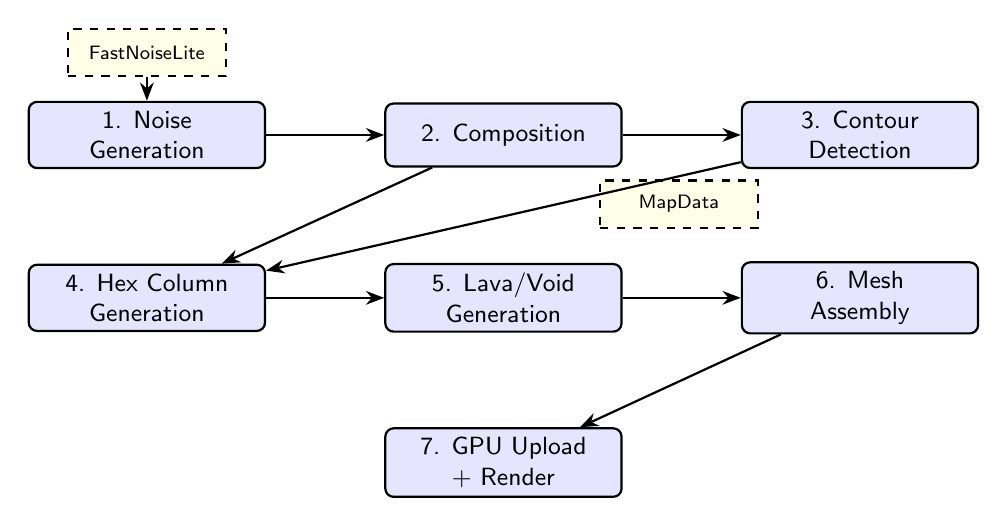
\begin{tikzpicture}[
  stage/.style={rectangle, draw, rounded corners=3pt, fill=blue!10,
                minimum width=3cm, minimum height=0.8cm, align=center,
                font=\small\sffamily},
  data/.style={rectangle, draw, dashed, fill=yellow!10,
               minimum width=2cm, minimum height=0.6cm, align=center,
               font=\scriptsize\sffamily},
  >=Stealth, thick
]
  \node[stage] (noise) {1. Noise\\Generation};
  \node[stage, right=1.5cm of noise] (comp) {2. Composition};
  \node[stage, right=1.5cm of comp] (cont) {3. Contour\\Detection};
  \node[stage, below=1.2cm of noise] (hex) {4. Hex Column\\Generation};
  \node[stage, right=1.5cm of hex] (lava) {5. Lava/Void\\Generation};
  \node[stage, right=1.5cm of lava] (mesh) {6. Mesh\\Assembly};
  \node[stage, below=1.2cm of lava] (gpu) {7. GPU Upload\\+ Render};

  \node[data, above=0.3cm of noise] (fnl) {FastNoiseLite};
  \node[data, below right=0.15cm and -0.3cm of comp] (md) {MapData};

  \draw[->] (noise) -- (comp);
  \draw[->] (comp) -- (cont);
  \draw[->] (cont) -- (hex);
  \draw[->] (comp) -- (hex);
  \draw[->] (hex) -- (lava);
  \draw[->] (lava) -- (mesh);
  \draw[->] (mesh) -- (gpu);
  \draw[->] (fnl) -- (noise);
\end{tikzpicture}
\caption{Terrain pipeline data flow}
\label{fig:terrain-pipeline}
\end{figure}

\subsection{Step 1: Noise Generation}
\label{sec:noise}

\texttt{noise.h/cpp} and \texttt{noise\_layers.cpp} generate three noise layers using FastNoiseLite.

\subsubsection{Elevation Layer}

\begin{lstlisting}[caption={NoiseParams defaults}]
struct NoiseParams {
  float frequency = 0.003f;
  int   octaves = 6;
  float lacunarity = 2.0f;
  float gain = 0.5f;
  int   seed = 1337;
  int   terrace_levels = 8;
  int   min_region_size = 153;
};
\end{lstlisting}

\textbf{Algorithm} --- Multi-octave OpenSimplex2 with gradient-based erosion:

\begin{lstlisting}[caption={Gradient erosion pseudocode},numbers=none]
for each octave i:
  octave[x] = noise.GetNoise(x * map_scale, y * map_scale)
  grad_mag = sqrt(gradient_x[x]^2 + gradient_y[x]^2)
  erosion_factor = 1.0 / (1.0 + grad_mag * GRADIENT_SCALE)  // GRADIENT_SCALE = 2.0
  out[x] += octave[x] * amplitude * erosion_factor
  // Update gradient accumulator
  dx = (octave[x+1] - octave[x-1]) * 0.5
  gradient_x[x] += dx * amplitude * erosion_factor * frequency
  amplitude *= gain;  frequency *= lacunarity
\end{lstlisting}

Post-processing: normalize to $[0,1]$, apply \texttt{biased\_smoothstep} (blend of Hermite $3t^2-2t^3$ and quadratic ease-out $1-(1-t)^2$, controlled by \texttt{scurve\_bias}), then terrace: $\lfloor v \cdot L \rfloor / L$.

\subsubsection{River Mask}

Uses \texttt{FractalType\_Ridged} with OpenSimplex2 (frequency 0.008, 4 octaves). The ridged fractal creates natural river-vein patterns. Output is min-max normalized across the entire map.

\subsubsection{Worley (Cellular) Layer}

\begin{lstlisting}[caption={WorleyParams defaults}]
struct WorleyParams {
  float frequency = 0.015f;
  float jitter = 1.0f;
  float warp_amp = 40.0f;       // domain warp amplitude
  float warp_frequency = 0.003f;
  int   warp_octaves = 3;
};
\end{lstlisting}

Three simultaneous outputs from one cellular noise evaluation:
\begin{enumerate}
  \item \textbf{Distance} (\texttt{EuclideanSq}, \texttt{Distance}) --- distance to nearest cell center
  \item \textbf{Edge} (\texttt{Distance2Sub}) --- difference between 1st and 2nd nearest distances
  \item \textbf{Cell Value} (\texttt{CellValue}) --- per-cell random ID
\end{enumerate}

\textbf{Domain warp:} A separate FastNoiseLite instance (\texttt{seed + 31337}) with \texttt{DomainWarpType\_OpenSimplex2} and \texttt{FractalType\_DomainWarpProgressive} distorts the input coordinates before Worley evaluation, creating organic Voronoi boundary distortion.

\begin{howtip}
FastNoiseLite key calls: \texttt{SetNoiseType()}, \texttt{SetFrequency()}, \texttt{SetFractalType()}, \texttt{SetFractalOctaves/Lacunarity/Gain()}, \texttt{SetCellularDistanceFunction()}, \texttt{SetCellularReturnType()}, \texttt{SetCellularJitter()}, \texttt{SetDomainWarpType()}, \texttt{SetDomainWarpAmp()}, \texttt{DomainWarp(wx, wy)}, \texttt{GetNoise(x, y)}.
\end{howtip}

\subsection{Step 2: Composition}
\label{sec:composition}

\texttt{noise\_composer.cpp} blends the three noise layers into the final terrain.

\textbf{NoiseCache:} A 3-slot cache using FNV-1a hashing of parameter structs. Avoids regenerating noise layers when only composition parameters change during ImGui tweaking.

\textbf{Pipeline:}
\begin{enumerate}
  \item Copy elevation $\to$ \texttt{final\_elevation}
  \item Terrace: \texttt{basalt\_height[i] = floor(elev[i] * levels) / levels}
  \item \texttt{cleanup\_small\_regions()}: flood-fill regions of matching \texttt{basalt\_height} ($\pm$0.01 threshold); if region $<$ \texttt{min\_region\_size}, replace with 3$\times$3 neighbor average
\end{enumerate}

\subsection{Step 3: Contour Detection}
\label{sec:contour}

\texttt{contour.cpp} extracts elevation contour lines and detects plateaus.

\subsubsection{Marching Squares}

\begin{lstlisting}[caption={Marching squares pseudocode},numbers=none]
for each cell (x, y), for each level L from interval/2 to 1.0:
  config = 4-bit mask of corners >= L
  if config in {0, 15}: skip (all above or below)
  // 2-point cases: interpolate crossing position on edges
  // 4-point cases (saddle): check cell center height to resolve
  emit Line{x1, y1, x2, y2, elevation=L}
\end{lstlisting}

Hard cap: \texttt{MAX\_CONTOUR\_LINES = 500{,}000}. Post-processing: \texttt{simplify\_contours()} removes segments with squared length $< \varepsilon^2$.

\subsubsection{Plateau Detection}

BFS flood-fill on \texttt{band\_map} (discrete elevation bands). Each plateau stores: pixel list, center of mass, bounding box, average height. Filter: only plateaus with $>50$ pixels are retained.

\begin{lstlisting}[caption={Plateau structure}]
struct Plateau {
  float height;
  std::vector<int> pixels;
  float center_x, center_y;
  float min_x, max_x, min_y, max_y;
};
\end{lstlisting}

\subsection{Step 4: Hex Column Generation}
\label{sec:hex}

\subsubsection{Axial Hex Coordinates}

\texttt{hex.h/cpp} implements pointy-top hexagonal grids with axial coordinates $(q, r)$.

\begin{align}
  \text{hex\_to\_pixel:} \quad x &= s \cdot 1.5 \cdot q, \quad y = s \cdot \sqrt{3} \cdot (r + 0.5q) \\
  \text{pixel\_to\_hex:} \quad q &= \tfrac{2}{3} \cdot x / s, \quad r = (-\tfrac{1}{3} \cdot x + \tfrac{\sqrt{3}}{3} \cdot y) / s
\end{align}

Pixel-to-hex uses \textbf{cubic rounding}: convert to cube coordinates $(q, r, s=-q-r)$, round each, then fix the axis with the largest rounding error to maintain the $q+r+s=0$ constraint.

\textbf{Hex corners:} 6 vertices at angles $i \cdot \pi/3$ for $i \in [0,6)$, offset from hex center by \texttt{hex\_size}. Point-in-hex test uses 6 half-plane cross-product checks.

\subsubsection{Column Generation (\texttt{basalt.cpp})}

Two generation strategies exist:

\textbf{V1 (Plateau-based):} For each plateau ($\geq$300 pixels, aspect ratio $\leq$3.0), find center hex, BFS-expand outward. Each candidate hex is tested by checking a 3$\times$3 pixel bounding box against \texttt{terrain\_map}. Height variation: $\pm$0.025 via \texttt{hash(q,r)}.

\textbf{V2 (Worley-based):} Iterate all hexes in map bounds. Per hex: jitter position via hash, check \texttt{worley\_cell\_value} against \texttt{density\_threshold} (default 0.2), skip if in \texttt{liquid\_mask}. Height from base elevation plus cell-value jitter.

\textbf{Visible edges:} \texttt{compute\_visible\_edges()} checks each of 6 hex neighbors (offset table: $(1,0), (0,1), (-1,1), (-1,0), (0,-1), (1,-1)$). An edge is visible if the neighbor is absent or lower by $>$0.01.

\subsection{Step 5: Lava/Void Generation}
\label{sec:lava}

\texttt{lava.cpp} flood-fills non-basalt regions to create lava and void bodies.

\textbf{Budget caps:}
\begin{itemize}
  \item \texttt{MAX\_COMPONENT\_PIXELS = 50{,}000} per body
  \item \texttt{TOTAL\_PIXEL\_BUDGET = 200{,}000} global
  \item Minimum component size: 50 pixels
\end{itemize}

Each component is randomly classified as void (30\% chance) or lava (70\%). Lava bodies get a mesh: a sparse grid (2.0 unit spacing) with 2 triangles per quad cell. Grid size capped at \texttt{MAX\_LAVA\_GRID\_CELLS = 40{,}000}. Each body gets a random time offset for wave animation phase: $\text{offset} = (\text{hash}(\text{idx}) \bmod 1000) / 1000 \cdot 2\pi$.

\subsection{Step 6: Mesh Assembly}
\label{sec:mesh}

\texttt{terrain\_mesh.cpp} converts terrain data into GPU-ready vertex/index buffers.

\begin{table}[h]
\centering
\caption{Vertex format layouts}
\label{tab:vertices}
\begin{tabular}{@{}llrl@{}}
\toprule
\textbf{Struct} & \textbf{Fields} & \textbf{Size} & \textbf{Usage} \\
\midrule
BasaltVertex  & pos(3), color(3), sheen(1), normal(3) & 48\,B & Hex columns \\
GpuLavaVertex & pos(3), time\_offset(1) & 16\,B & Lava surfaces \\
ContourVertex & pos(3) & 12\,B & Contour lines \\
\bottomrule
\end{tabular}
\end{table}

\textbf{Two-layer basalt mesh:}
\begin{itemize}
  \item \textbf{Layer 0 (sides):} Per visible edge, 4 vertices (top-near, top-far, bottom-far, bottom-near) and 2 triangles. Normal computed as 2D perpendicular to the edge direction. Side sheen = $\text{sheen} \times 0.4$.
  \item \textbf{Layer 1 (tops):} 6 vertices per hexagon + 4 fan triangles from vertex 0. Normal = $(0, 0, 1)$.
\end{itemize}

Color is generated by \texttt{organic\_color()}: palette interpolation based on elevation with per-hex hash noise for variation.

\subsection{Step 7: GPU Upload \& Rendering}
\label{sec:terrain-render}

\texttt{terrain\_renderer.cpp} manages five GPU pipelines and the draw order.

% ── Render Pass Order Diagram ──
\begin{figure}[h]
\centering
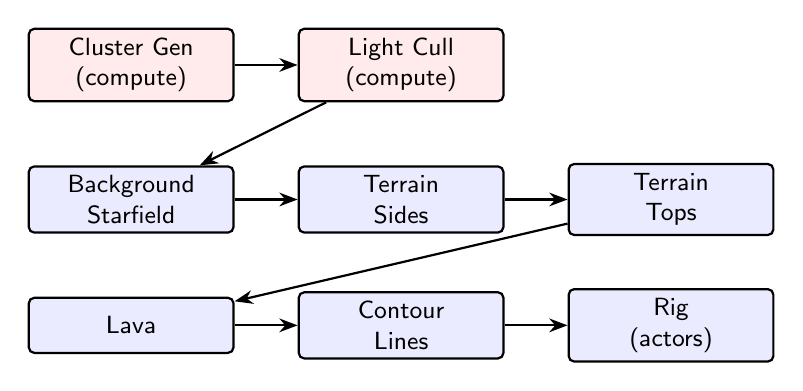
\begin{tikzpicture}[
  pass/.style={rectangle, draw, rounded corners=2pt, fill=blue!8,
               minimum width=2.6cm, minimum height=0.7cm, align=center,
               font=\small\sffamily},
  comp/.style={rectangle, draw, rounded corners=2pt, fill=red!8,
               minimum width=2.6cm, minimum height=0.7cm, align=center,
               font=\small\sffamily},
  >=Stealth, thick
]
  \node[comp] (clust) {Cluster Gen\\(compute)};
  \node[comp, right=0.8cm of clust] (cull) {Light Cull\\(compute)};
  \node[pass, below=0.8cm of clust] (bg) {Background\\Starfield};
  \node[pass, right=0.8cm of bg] (sides) {Terrain\\Sides};
  \node[pass, right=0.8cm of sides] (tops) {Terrain\\Tops};
  \node[pass, below=0.8cm of bg] (lava) {Lava};
  \node[pass, right=0.8cm of lava] (cont) {Contour\\Lines};
  \node[pass, right=0.8cm of cont] (rig) {Rig\\(actors)};

  \draw[->] (clust) -- (cull);
  \draw[->] (cull) -- (bg);
  \draw[->] (bg) -- (sides);
  \draw[->] (sides) -- (tops);
  \draw[->] (tops) -- (lava);
  \draw[->] (lava) -- (cont);
  \draw[->] (cont) -- (rig);
\end{tikzpicture}
\caption{Render pass execution order}
\label{fig:render-order}
\end{figure}

\textbf{Clustered light culling} (compute pass before rendering):
\begin{itemize}
  \item \texttt{generate\_clusters.comp}: $16 \times 9$ tile grid $\times$ 24 depth slices = 3456 clusters. Computes view-space AABB per cluster.
  \item \texttt{light\_culling.comp}: sphere--AABB intersection test per light per cluster. Outputs light grid + global index list (max 65536 indices, max 1024 lights).
  \item Cluster index: $\texttt{tileX} + \texttt{tileY} \times \texttt{gridX} + \texttt{slice} \times \texttt{gridX} \times \texttt{gridY}$
\end{itemize}

\textbf{SceneUniforms} (std140, pushed per draw call): view/projection matrices, time, contour opacity, lava color, star light (RGB + intensity), directional light (direction + color + ambient), grid parameters for clustering, near/far planes, light count.

% ══════════════════════════════════════════════════════════════════════
\section{Shader Architecture}
\label{sec:shaders}

All shaders are GLSL~4.5, compiled to SPIR-V. Three shared includes define common interfaces.

\subsection{Shared Includes}

\textbf{\texttt{coord.glsl}} --- \texttt{SceneUniforms} UBO (set=1, binding=0) and the \texttt{cluster\_index()} function that maps fragment position to a 3D cluster cell.

\textbf{\texttt{lighting\_common.glsl}} --- \texttt{PointLight} (32\,B: pos+radius, color+intensity), \texttt{ClusterAABB} (min/max vec4), \texttt{LightGridEntry} (offset + count).

\textbf{\texttt{pbr\_common.glsl}} --- Cook-Torrance BRDF:
\begin{align}
  D_\text{GGX}(h) &= \frac{\alpha^2}{\pi\bigl((\mathbf{n}\cdot\mathbf{h})^2(\alpha^2-1)+1\bigr)^2} \\
  G_\text{Schlick}(v) &= \frac{\mathbf{n}\cdot\mathbf{v}}{(\mathbf{n}\cdot\mathbf{v})(1-k)+k}, \quad k = \frac{(\alpha+1)^2}{8} \\
  F_\text{Schlick}(\theta) &= F_0 + (1-F_0)(1-\cos\theta)^5, \quad F_0 = \text{mix}(0.04, \text{albedo}, \text{metallic})
\end{align}

\subsection{Terrain Shaders}

\textbf{Vertex:} Transforms position by view $\times$ projection. Passes color, normal, world position, sheen.

\textbf{Fragment:} Lambertian diffuse from directional light + star ambient + clustered point lights. Applies a hex dither function for subtle per-cell color variation:
\begin{lstlisting}[style=glslstyle,numbers=none]
// Hash hex cell center for dither
uint h = uint(iq) * 374761393u ^ uint(ir) * 668265263u;
float dither = (float(h & 0xFFu) / 255.0 - 0.5) * 0.25;
\end{lstlisting}

\subsection{Lava Shaders}

\textbf{Vertex:} Triple sine-wave deformation for animated surface:
\begin{lstlisting}[style=glslstyle,numbers=none]
float t = time + time_offset;
float wave = sin(pos.x * 0.3 + t) * 0.02
           + sin(pos.y * 0.21 + t * 1.3) * 0.015
           + sin((pos.x + pos.y) * 0.15 + t * 0.8) * 0.01;
pos.z += wave;
\end{lstlisting}

\textbf{Fragment:} Depth-based darkening: \texttt{depth\_factor = clamp(0.9 + wave * 2.0, 0.8, 1.1)}.

\subsection{Background Shaders}

Full-screen triangle (vertex ID only, no VBO). Fragment generates a procedural starfield:
\begin{itemize}
  \item 3 layers with cell sizes 120, 55, 28 pixels and spawn chances 0.45, 0.38, 0.30
  \item Per-star: hash-based position + twinkle (frequency 0.5--2.5\,Hz, random phase)
  \item Core radius 0.3--0.7\,px, glow = 3.5$\times$ core radius
  \item Radiance: $e^{-d^2/r^2}$, luminance 0.25--1.0
  \item Parallax scroll at 0.18$\times$ camera speed
\end{itemize}

\subsection{Contour Shaders}

Simple pass-through vertex shader. Fragment outputs a fixed color with configurable alpha. Blending: src-alpha / one-minus-src-alpha. No depth test or write---contours overlay everything.

\subsection{Compute Shaders}

Both use \texttt{local\_size = (16, 9, 1)} matching the tile grid dimensions.

\textbf{Cluster generation:} Converts each tile + depth slice to a view-space AABB using inverse projection. Stores min/max bounds per cluster.

\textbf{Light culling:} For each cluster, tests all lights for sphere--AABB intersection. Writes matching light indices into a global index buffer with an atomic counter.

\subsection{Instanced Terrain}

SSBO at set=0 contains \texttt{ColumnInstance} (80\,B: mat4 model + vec4 color). Vertex shader reads instance data by \texttt{gl\_InstanceIndex}. Normal transform uses the inverse-transpose of the model matrix upper-left 3$\times$3.

\subsection{PBR Static}

Drop-in replacement for the terrain pipeline. Uses Cook-Torrance BRDF from \texttt{pbr\_common.glsl} with clustered lighting fallback (iterates all lights if cluster lookup fails).

% ══════════════════════════════════════════════════════════════════════
\section{Procedural Animation System (Rig System)}
\label{sec:animation}

The rig system provides fully procedural character animation---no pre-baked animations, no motion capture. Everything is computed per-frame from physics and locomotion state.

\subsection{Skeleton}

\texttt{rig.h} defines a 32-joint skeleton:

\begin{table}[h]
\centering
\caption{Joint hierarchy (32 joints, \texttt{Joint::COUNT = 32})}
\label{tab:joints}
\begin{tabular}{@{}lp{9cm}@{}}
\toprule
\textbf{Group} & \textbf{Joints} \\
\midrule
Core spine (8) & ROOT, HIPS, SPINE\_01, SPINE\_02, CHEST, NECK, HEAD, HEAD\_END \\
Left arm (4)   & L\_CLAVICLE, L\_UPPER\_ARM, L\_LOWER\_ARM, L\_HAND \\
Right arm (4)  & R\_CLAVICLE, R\_UPPER\_ARM, R\_LOWER\_ARM, R\_HAND \\
Left leg (4)   & L\_UPPER\_LEG, L\_LOWER\_LEG, L\_FOOT, L\_TOE \\
Right leg (4)  & R\_UPPER\_LEG, R\_LOWER\_LEG, R\_FOOT, R\_TOE \\
IK virtual (8) & POLE\_KNEE\_L/R, POLE\_ELBOW\_L/R, IK\_FOOT\_L/R, IK\_HAND\_L/R \\
\bottomrule
\end{tabular}
\end{table}

\textbf{ActorConfig} defines anthropomorphic proportions (all scaled by 0.85$\times$ reference):
\begin{itemize}
  \item Legs: \texttt{leg\_len=0.366}, \texttt{shin\_len=0.332}
  \item Torso: \texttt{torso\_len=0.520}, \texttt{neck\_len=0.104}
  \item Arms: \texttt{arm\_len=0.270}, \texttt{forearm\_len=0.230}
  \item Widths: \texttt{hip\_width=0.25}, \texttt{shoulder\_width=0.35}
  \item \texttt{ISO\_VERT\_SCALE = 0.8165} (isometric Z compression)
\end{itemize}

\texttt{RigPose} holds world-space \texttt{vec3 joints[32]}. Derived joints (ROOT, SPINE\_02, HEAD\_END, clavicles, toes, pole targets, IK goals) are computed in SkeletonFinalise.

\subsection{ECS System Pipeline}
\label{sec:systems}

Nine systems registered as \texttt{flecs::PostUpdate}, executed in strict order.

% ── ECS System Order Diagram ──
\begin{figure}[h]
\centering
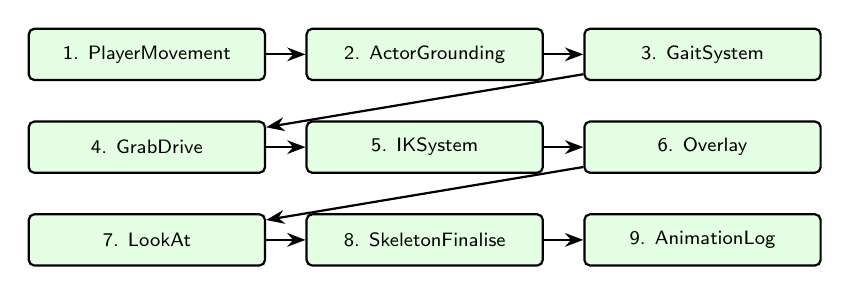
\begin{tikzpicture}[
  sys/.style={rectangle, draw, rounded corners=2pt, fill=green!10,
              minimum width=3cm, minimum height=0.65cm, align=center,
              font=\scriptsize\sffamily},
  >=Stealth, thick
]
  \node[sys] (s1) {1. PlayerMovement};
  \node[sys, right=0.5cm of s1] (s2) {2. ActorGrounding};
  \node[sys, right=0.5cm of s2] (s3) {3. GaitSystem};
  \node[sys, below=0.5cm of s1] (s4) {4. GrabDrive};
  \node[sys, right=0.5cm of s4] (s5) {5. IKSystem};
  \node[sys, right=0.5cm of s5] (s6) {6. Overlay};
  \node[sys, below=0.5cm of s4] (s7) {7. LookAt};
  \node[sys, right=0.5cm of s7] (s8) {8. SkeletonFinalise};
  \node[sys, right=0.5cm of s8] (s9) {9. AnimationLog};

  \draw[->] (s1) -- (s2);
  \draw[->] (s2) -- (s3);
  \draw[->] (s3) -- (s4);
  \draw[->] (s4) -- (s5);
  \draw[->] (s5) -- (s6);
  \draw[->] (s6) -- (s7);
  \draw[->] (s7) -- (s8);
  \draw[->] (s8) -- (s9);
\end{tikzpicture}
\caption{Animation ECS system execution order}
\label{fig:ecs-order}
\end{figure}

\subsubsection{1. PlayerMovementSystem}

Maps WASD input to isometric movement axes (45$^\circ$ rotation: $\cos 45^\circ = \sin 45^\circ = 0.707$). Velocity smoothed via \texttt{SmoothDamp} with \texttt{smooth\_time=0.1s}. Facing updated via \texttt{atan2} when speed $> 0.001$. Turn detection uses hysteresis: enter large-turn at $>60^\circ$, exit at $<20^\circ$. Visual facing has adaptive smooth time: 0.15\,s (small turns) to 0.50\,s (full reversal). Chest facing lags with 0.22\,s (moving) or 0.06\,s (idle).

\subsubsection{2. ActorGroundingSystem}

Snaps actor Z to terrain height via bilinear sampling of \texttt{final\_elevation}.

\subsubsection{3. GaitSystem --- Distance-Based Procedural Stepping}

The gait system is the most complex animation subsystem. It maintains a one-foot-planted invariant: exactly one foot is always grounded while the other may be stepping.

\textbf{Key parameters:} \texttt{stride\_len=0.85}, \texttt{step\_height=0.16}, \texttt{step\_duration=0.25s}, \texttt{SWING\_RATE=2.7\,rad/s}.

\textbf{Phase accumulation:} \texttt{phase += speed * dt * SWING\_RATE}

\textbf{Unified step basis:} The step direction is derived from a blend of velocity direction and visual facing (max 70\% blend during turns). Both \texttt{step\_fwd} and \texttt{step\_rght} are computed from this unified basis, preventing asymmetric reach during turns.

\textbf{Step triggering:} A step is triggered when the planted foot's distance from the hip socket exceeds \texttt{trigger\_dist = half\_stride * (0.25 + 0.75 * speed\_factor)}. Half-space constraint forces corrective steps when a foot crosses the center line.

\textbf{Foot placement (velocity-predicted):}
\[\text{target\_off} = (\text{half\_stride} + \text{speed} \cdot \text{duration} \cdot 0.75) \cdot \text{speed\_factor}\]

\textbf{Foot animation:}
\begin{itemize}
  \item XY: smootherstep $t^3(10t^2 - 15t + 6)$ interpolation
  \item Z: $t^2(3-2t) + \sin(\pi t) \cdot \text{step\_height}$ (parabolic arc)
\end{itemize}

\textbf{Turn-aware sequencing:} The trailing foot (relative to turn direction) steps first when \texttt{turn\_urgency $>$ 0.4}. Starvation guard resets the queue when urgency drops below 0.4.

\subsubsection{4. GrabDriveSystem}

Maps \texttt{GrabState} to \texttt{ArmIKGoal} targets. Activates \texttt{HeavyCarry} overlay and reduces stride when carrying objects.

\subsubsection{5. IKSystem --- Two-Bone Analytical IK}

\textbf{Spine FK} builds the chain bottom-up: HIPS $\to$ SPINE\_01 $\to$ CHEST $\to$ NECK $\to$ HEAD, using torso segment lengths.

\textbf{Arm swing (FK pendulum):} Swing amplitude = $\min(1, \text{speed}/\text{move\_speed}) \times 30^\circ$. Left and right arms are anti-phase: $l = \sin(\phi + \pi)$, $r = \sin(\phi)$. Joint delay chain for successive breaking: shoulder 0.02\,s, elbow 0.04\,s, wrist 0.06\,s smooth-damp times. Rotation applied via Rodriguez formula around the chest-right axis.

\textbf{Two-bone IK solver:}
\begin{lstlisting}[caption={Two-bone analytical IK}]
void solve_two_bone(vec3 H, vec3 target, float a, float b,
                    vec3 pole, vec3 fallback_perp,
                    vec3 &out_mid, vec3 &out_end) {
  float D = clamp(length(target - H), |a-b|+0.001, a+b-0.001);
  float cos_alpha = (a*a + D*D - b*b) / (2*a*D);  // law of cosines
  vec3 dir = normalize(target - H);
  vec3 perp = normalize(pole_projected);  // or fallback_perp
  out_mid = H + (dir * cos_alpha + perp * sin_alpha) * a;
  out_end = target;
}
\end{lstlisting}

Per-leg fallback perpendiculars: left knee gets $(-\text{rght})$, right gets $(+\text{rght})$, preventing shared fallback from pushing both knees the same direction.

\subsubsection{6. OverlaySystem --- Additive Overlays}

Three overlay types applied additively to the pose:
\begin{itemize}
  \item \textbf{Limp:} Asymmetric left hip drop: $\sin(\phi) \times 0.04 \times \text{intensity}$
  \item \textbf{Fatigue:} Increased sway + forward lean (0.03 rad) + slow breathing
  \item \textbf{HeavyCarry:} Forward lean (0.05 rad) + pulled-down hands ($-0.06 \times \text{intensity}$)
\end{itemize}

\subsubsection{7. LookAtSystem --- Head Tracking}

Decomposes target direction into yaw/pitch relative to facing. Clamped: yaw $\in [-70^\circ, 70^\circ]$, pitch $\in [-30^\circ, 30^\circ]$. SmoothDamp with 0.08\,s. Distribution: HEAD 60\%, NECK 30\%, CHEST 10\%.

\subsubsection{8. SkeletonFinaliseSystem}

The most complex system, performing multiple physics-driven corrections:

\textbf{Slope hip tilt:} From foot height difference, clamped $\pm 8^\circ$. Applied to hip socket Z as $\sin(\text{tilt}) \times \text{hip\_width}$.

\textbf{CoM hip sway:} Support balance $\in [-1, +1]$ smoothed with 0.08\,s. Lateral displacement = $\text{balance} \times 0.04$.

\textbf{Hip counter-animation:}
\begin{align}
  \text{hip\_roll} &= \sin(\phi) \times 0.06 \times \text{walk\_blend} \\
  \text{hip\_bob}  &= |\sin(\phi)| \times 0.018 \times \text{walk\_blend} \times (1 - \text{turn\_urgency} \times 0.7) \\
  \text{hip\_dip}  &= 4p(1-p) \times (\text{leg\_len} + \text{shin\_len}) \times 0.07 \quad \text{(parabolic during swing)}
\end{align}

\textbf{Acceleration-driven torso lean:} lean factor = $\min(|\mathbf{a}| \times 0.015, 8^\circ)$, with additional 2.5$^\circ$ forward lean when moving. Applied via successive breaking to chest (0.05\,s), neck (0.08\,s), head (0.12\,s).

\textbf{Idle micro-motion:} Breathing at 0.6\,Hz (amplitude 0.008), lateral sway at 0.15\,Hz (amplitude 0.01), weight shift at 0.3\,Hz (hip shift 0.04, dip 0.012). All scaled by $\text{idle\_blend} = 1 - \min(1, \text{speed}/0.2)$.

\subsubsection{9. AnimationLogSystem}

Outputs JSONL telemetry per frame: transform, velocity, gait phase, all 32 joint positions, arm swing diagnostics, spine offsets, grounding state.

\subsection{SmoothDamp --- Critically Damped Spring}
\label{sec:smoothdamp}

\begin{lstlisting}[caption={SmoothDamp implementation (Unity-compatible)}]
float smooth_damp(float current, float target, float *velocity,
                  float smooth_time, float dt) {
  float omega = 2.0f / smooth_time;
  float x     = omega * dt;
  float exp_f = 1.0f / (1 + x + 0.48f*x*x + 0.235f*x*x*x);
  float delta = current - target;
  float temp  = (*velocity + omega * delta) * dt;
  *velocity   = (*velocity - omega * temp) * exp_f;
  return target + (delta + temp) * exp_f;
}
\end{lstlisting}

The angle-aware variant wraps \texttt{delta} to $[-\pi, \pi]$ before smoothing.

% ══════════════════════════════════════════════════════════════════════
\section{Rig Renderer}
\label{sec:rig-render}

\texttt{rig\_renderer.cpp} generates procedural bone-cage meshes entirely at runtime---no pre-baked geometry.

\textbf{Vertex budget:} 65{,}536 vertices per frame (2.5\,MB persistent transfer buffer).

\textbf{Emit functions:}
\begin{itemize}
  \item \texttt{emit\_cylinder()} --- $n$-sided cylinder with computed normals
  \item \texttt{emit\_bone\_oct()} --- tapered octahedron (4 sides, 20\% equator), classic rig viz
  \item \texttt{emit\_sphere()} --- UV sphere (sectors $\times$ rings)
  \item \texttt{emit\_box()} --- 6-face solid cube
  \item \texttt{emit\_diamond()} --- 6-vertex octahedron (8 triangles)
  \item \texttt{emit\_flat\_circle()} --- fan-triangulated disc on XY plane
\end{itemize}

\textbf{Isometric compensation} adjusts bone rendering for the isometric view:
\begin{align}
  \text{width\_scale} &= 1.0 + \sqrt{|\mathbf{d} \cdot \hat{z}|} \times 2.0 \quad \in [1, 3] \\
  \text{equator\_t} &= 0.2 + |\mathbf{d} \cdot \hat{z}| \times 0.15 \\
  \text{radial\_z\_comp} &= 0.18 + |\mathbf{d} \cdot \hat{z}| \times 0.82
\end{align}

Where $\mathbf{d}$ is the bone direction. Bones pointing more vertically get wider cross-sections to remain visible under isometric foreshortening.

\textbf{Body part rendering:} Spine (4 segments, 6-sided, radii 1.3--1.4$\times$), head (2 segments, taper 0.4--0.3$\times$), legs (4 segments each, 1.4--0.3$\times$), arms (4 segments each, 1.5--0.75$\times$).

\textbf{Debug shapes:} IK goals as green boxes (0.04 half-size), pole targets as orange diamonds (0.04 radius), pole lines as dashed orange cylinders.

% ══════════════════════════════════════════════════════════════════════
\section{glTF Asset Pipeline}
\label{sec:gltf-pipeline}

\subsection{Loading Pipeline}

\texttt{load\_gltf(path)} uses cgltf for parsing and stb\_image for textures:

\begin{enumerate}
  \item \texttt{cgltf\_parse\_file()} --- parse the .glb/.gltf file
  \item \texttt{cgltf\_load\_buffers()} --- load binary buffer data
  \item \texttt{cgltf\_validate()} --- validate the asset
  \item Extract mesh attributes via \texttt{cgltf\_accessor\_read\_float/uint()}
  \item Decode embedded textures via \texttt{stbi\_load\_from\_memory()}
\end{enumerate}

Returns \texttt{GltfAsset} containing vectors of \texttt{GltfMeshData} (vertices + indices) and \texttt{GltfTextureData} (RGBA pixels, sRGB flag).

\subsection{Instanced Terrain Rendering}

\texttt{instanced\_terrain.h/cpp} renders glTF column meshes via GPU instancing:

\begin{lstlisting}[caption={ColumnInstance layout (80 bytes)}]
struct ColumnInstance {
  glm::mat4 model;     // 64B: translate(q,r) * scale(1,1,height)
  float color_r, color_g, color_b, color_a;  // 16B
};
\end{lstlisting}

Instances stored in an SSBO (\texttt{GRAPHICS\_STORAGE\_READ}). The vertex shader reads instance data by \texttt{gl\_InstanceIndex}. Toggle via \texttt{terrain\_renderer.use\_instanced} (ImGui checkbox).

% ══════════════════════════════════════════════════════════════════════
\section{ECS Architecture}
\label{sec:ecs}

Delve uses Flecs v4.0.5 for entity-component-system organization. All animation systems are registered as \texttt{flecs::PostUpdate} phase.

\subsection{Component Catalog}

\begin{table}[h]
\centering
\caption{ECS components on the player entity}
\label{tab:components}
\begin{tabular}{@{}lp{8cm}@{}}
\toprule
\textbf{Component} & \textbf{Purpose} \\
\midrule
\texttt{ActorTag}         & Tag component for entity queries \\
\texttt{Transform}        & Position (x, y, z) + facing angle \\
\texttt{Velocity}         & Movement velocity (x, y, z) \\
\texttt{ActorConfig}      & Skeletal proportions (bone lengths, radii) \\
\texttt{ProceduralGait}   & Gait phase, stride length, step height/duration \\
\texttt{LegState}         & Per-leg foot positions, stepping flags, plant positions \\
\texttt{RigPose}          & 32 world-space joint positions \\
\texttt{RigState}         & Animation smoothing state (velocity, lean, sway, etc.) \\
\texttt{LookAtTarget}     & Head tracking target position \\
\texttt{ArmIKGoal}        & Arm IK target positions + blend weights \\
\texttt{AnimationOverlay} & Additive overlay type (None/Limp/Fatigue/HeavyCarry) \\
\texttt{GrabState}        & Object grab state for arm IK \\
\bottomrule
\end{tabular}
\end{table}

\subsection{System Registration Pattern}

\begin{lstlisting}[caption={Flecs system registration}]
ecs.system<Transform, Velocity, ActorConfig, ProceduralGait,
           LegState, RigPose, RigState>("GaitSystem")
   .kind(flecs::PostUpdate)
   .run([](flecs::iter &it) {
     while (it.next()) { /* system logic */ }
   });
\end{lstlisting}

All 9 animation systems are registered in \texttt{register\_rig\_systems()} with explicit ordering via Flecs phase dependencies.

% ══════════════════════════════════════════════════════════════════════
\section{Testing Framework}
\label{sec:testing}

\subsection{Test Harness}

\texttt{src/test/test\_harness.h} provides a lightweight custom test framework.

\textbf{Registration:} \texttt{DELVE\_TEST(name) \{ ... return true; \}} --- creates a static function and registers it with \texttt{TestRegistry} at compile time.

\textbf{Assertion macros:}
\begin{table}[h]
\centering
\begin{tabular}{@{}lp{7cm}@{}}
\toprule
\textbf{Macro} & \textbf{Condition} \\
\midrule
\texttt{EXPECT\_TRUE(e)}      & \texttt{e} is truthy \\
\texttt{EXPECT\_FALSE(e)}     & \texttt{e} is falsy \\
\texttt{EXPECT\_NEAR(a,b,e)}  & $|a-b| \leq \varepsilon$ \\
\texttt{EXPECT\_RANGE(v,l,h)} & $l \leq v \leq h$ \\
\texttt{EXPECT\_GT/LT/GE/EQ}  & Relational comparisons \\
\bottomrule
\end{tabular}
\end{table}

\textbf{Output:} JSON to stdout: \texttt{\{"tests":[...], "passed":N, "failed":N, "total":N\}}.

\textbf{Headless testing:} SDL3 is stubbed out via headers in \texttt{src/test/sdl\_override/} that intercept includes. The \texttt{DELVE\_HEADLESS=1} compile definition disables GPU code paths.

\subsection{Metric Suites}

\textbf{Terrain metrics} (\texttt{terrain\_metrics.h}):
\begin{itemize}
  \item \texttt{elevation\_stats()} --- min, max, mean, stddev
  \item \texttt{water\_coverage\_percent(data, threshold=0.1)}
  \item \texttt{plateau\_count(band\_map)} --- max band ID
  \item \texttt{lava/void/basalt\_coverage\_ratio()} --- percentage of terrain\_map
\end{itemize}

\textbf{Geometry metrics} (\texttt{geometry\_metrics.h}):
\begin{itemize}
  \item \texttt{mesh\_degenerate\_triangles()} --- cross product magnitude $< 10^{-12}$
  \item \texttt{normal\_validity()} --- percentage with $|\|\mathbf{n}\| - 1| < 0.01$
  \item \texttt{hex\_roundtrip\_accuracy()} --- tests hex$\to$pixel$\to$hex roundtrip
\end{itemize}

\textbf{Animation metrics} (\texttt{animation\_metrics.h}):
\begin{itemize}
  \item \texttt{pose\_symmetry\_score()} --- compares 6 L/R joint pairs, returns $1/(1+\text{diff})$
  \item \texttt{foot\_contact\_velocity()} --- lower is better, 0 = perfect plant
  \item \texttt{arm\_phase\_opposition()} --- 1.0 if arms counter-phase to legs
  \item \texttt{lean\_acceleration\_correlation()} --- validates physics-driven lean
\end{itemize}

\subsection{Test Files}

9 test source files covering: noise generation, hex coordinates, animation, color palettes, full terrain pipeline, mesh integrity, coordinate system roundtrips, skeletal animation, and skinned characters.

% ══════════════════════════════════════════════════════════════════════
\section{Library Reference}
\label{sec:libref}

\begin{longtable}{@{}p{2.2cm}p{5.5cm}p{5.5cm}@{}}
\toprule
\textbf{Library} & \textbf{Key Functions Used} & \textbf{Purpose in Delve} \\
\midrule
\endhead
\textbf{SDL3} &
  \texttt{SDL\_CreateGPUDevice}, \texttt{SDL\_AcquireGPUSwapchainTexture}, \texttt{SDL\_CreateGPUGraphicsPipeline}, \texttt{SDL\_CreateGPUComputePipeline}, \texttt{SDL\_BeginGPURenderPass}, \texttt{SDL\_DrawGPUPrimitives}, \texttt{SDL\_DispatchGPUCompute}, \texttt{SDL\_PushGPUVertexUniformData}, \texttt{SDL\_BindGPUVertexStorageBuffers}, \texttt{SDL\_CreateWindow}, \texttt{SDL\_PollEvent} &
  Windowing, GPU device management, render pass control, draw calls, compute dispatch, uniform upload, event polling \\
\midrule
\textbf{Flecs} &
  \texttt{world::entity()}, \texttt{world::system()}, \texttt{entity::set<T>()}, \texttt{entity::add<T>()}, \texttt{system::kind()}, \texttt{system::run()}, \texttt{iter::field<T>()}, \texttt{world::progress()} &
  Entity creation, component attachment, system registration with phase ordering, per-frame system execution \\
\midrule
\textbf{GLM} &
  \texttt{glm::ortho}, \texttt{glm::normalize}, \texttt{glm::cross}, \texttt{glm::dot}, \texttt{glm::length}, \texttt{glm::mix}, \texttt{glm::clamp}, \texttt{glm::translate}, \texttt{glm::scale}, \texttt{glm::inverse}, \texttt{glm::transpose}, \texttt{glm::mat4}, \texttt{glm::vec3/vec4} &
  Orthographic projection, vector math, matrix transforms, isometric view construction, bone basis computation \\
\midrule
\textbf{FastNoiseLite} &
  \texttt{SetNoiseType(OpenSimplex2)}, \texttt{SetFrequency}, \texttt{SetFractalType(Ridged/None)}, \texttt{SetFractalOctaves/Lacunarity/Gain}, \texttt{SetCellularDistanceFunction(EuclideanSq)}, \texttt{SetCellularReturnType(Distance/Distance2Sub/CellValue)}, \texttt{SetCellularJitter}, \texttt{SetDomainWarpType(OpenSimplex2)}, \texttt{SetDomainWarpAmp}, \texttt{DomainWarp(x,y)}, \texttt{GetNoise(x,y)} &
  Elevation heightmap (multi-octave with erosion), ridged river mask, Worley cellular (3 outputs), domain warp for organic boundaries \\
\midrule
\textbf{ImGui} &
  \texttt{ImGui::Begin/End}, \texttt{SliderFloat/Int}, \texttt{ColorEdit3}, \texttt{Checkbox}, \texttt{Text}, \texttt{Separator}, \texttt{TreeNode}, \texttt{NewFrame}, \texttt{Render}, \texttt{GetDrawData} &
  Real-time parameter editor for noise, composition, display, and rendering settings \\
\midrule
\textbf{cgltf} &
  \texttt{cgltf\_parse\_file}, \texttt{cgltf\_load\_buffers}, \texttt{cgltf\_validate}, \texttt{cgltf\_accessor\_read\_float}, \texttt{cgltf\_accessor\_read\_uint}, \texttt{cgltf\_free} &
  glTF 2.0 parsing for static mesh loading (basalt column asset) \\
\midrule
\textbf{stb\_image} &
  \texttt{stbi\_load\_from\_memory}, \texttt{stbi\_image\_free} &
  Decode embedded glTF textures (base color, normal, ORM maps) \\
\midrule
\textbf{stb\_image\_write} &
  \texttt{stbi\_write\_png} &
  Frame capture: swapchain $\to$ PNG file \\
\midrule
\textbf{nlohmann/json} &
  \texttt{json::parse}, \texttt{json::dump}, \texttt{operator[]}, \texttt{value<T>()}, \texttt{contains()} &
  Config save/load (\texttt{config.json}), test JSON output, IPC message parsing, animation telemetry \\
\bottomrule
\end{longtable}

% ══════════════════════════════════════════════════════════════════════
\section{Entry Point \& Runtime Flow}
\label{sec:entry}

\texttt{src/game/main.cpp} installs signal handlers (SIGTERM, SIGINT $\to$ \texttt{g\_emergency\_shutdown}), parses command-line arguments via \texttt{parse\_agent\_args()}, creates a \texttt{TopoGame} instance, and calls \texttt{game.run(agent\_config)}.

\texttt{TopoGame} (subclass of \texttt{Application}) overrides the lifecycle hooks to:
\begin{enumerate}
  \item \textbf{on\_init:} Load \texttt{config.json}, generate initial terrain, upload meshes to GPU, create player entity with all 12 components, register all 9 animation systems
  \item \textbf{on\_render\_tool:} Draw ImGui parameter editor (noise, composition, display settings)
  \item \textbf{on\_render\_game:} Execute render pass order: compute (cluster gen $\to$ light cull) $\to$ background $\to$ terrain $\to$ lava $\to$ contours $\to$ rig
  \item \textbf{on\_event:} Forward to input system and ImGui
  \item \textbf{on\_cleanup:} Release GPU resources, save config
\end{enumerate}

Runtime configuration is persisted in \texttt{config.json} at the project root.

\end{document}
